\documentclass[12pt]{article}

% ---- Packages ----
\usepackage[margin=1in]{geometry}
\usepackage{times}
\usepackage{amsmath, amssymb}
\usepackage{graphicx}
\usepackage{enumitem}
\usepackage{tikz}
\usepackage{pgfplots}
\pgfplotsset{compat=1.18}
\usepackage{booktabs}
\usepackage{array}
\usepackage{multirow}
\usepackage{setspace}
\usepackage{parskip}
\usepackage{fancyhdr}
\usepackage{lastpage}
\usepackage{hyperref}

\hypersetup{
    colorlinks=false,
    pdfborder={0 0 0}
}

% ---- Page style ----
\pagestyle{fancy}
\fancyhf{}
\renewcommand{\headrulewidth}{0pt}
\fancyfoot[C]{\thepage}

% ---- Custom commands ----
\newcommand{\answerkey}[1]{\textbf{Answer: #1}}

\begin{document}

% ====================
% COVER PAGE
% ====================
\begin{titlepage}
\centering
\vspace*{3cm}

{\Huge\bfseries AP Statistics S2 Project}\\[0.8cm]
{\LARGE AP-Style Question Design \& Rubric Creation}\\[2.5cm]

{\Large
\begin{tabular}{rl}
\textbf{Student Name:} & Mickey Zhang (Zhang Jiamin) \\[0.5cm]
\textbf{Class Number:} & P1 \\[0.5cm]
\textbf{Date:} & April 2, 2026 \\
\end{tabular}
}

\vfill
{\large AP Statistics --- Semester 2}
\end{titlepage}

% ====================
% MULTIPLE CHOICE QUESTIONS
% ====================
\section*{Multiple-Choice Questions}

% ---- MCQ 1: Statistical Graph Question ----
\noindent\textbf{Question 1}

A city health department collected data on the number of hours of sleep per night for a random sample of 200 adults. The results are summarized in the histogram below.

\begin{center}
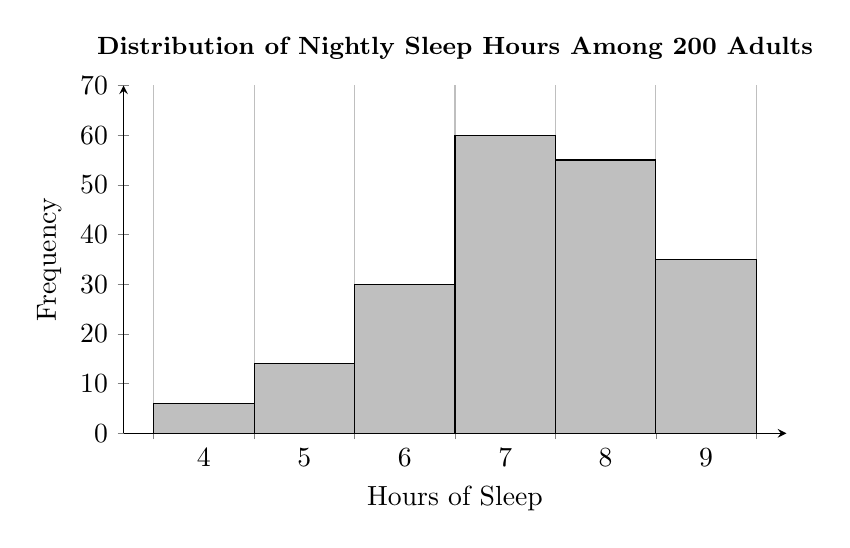
\begin{tikzpicture}
\begin{axis}[
    ybar interval,
    width=10cm, height=6cm,
    xlabel={Hours of Sleep},
    ylabel={Frequency},
    ymin=0, ymax=70,
    xtick={4,5,6,7,8,9,10},
    xticklabel style={anchor=north},
    ytick={0,10,20,30,40,50,60,70},
    axis lines=left,
    enlarge x limits=0.05,
    bar width=0.9,
    title={Distribution of Nightly Sleep Hours Among 200 Adults},
    title style={font=\bfseries\small},
]
\addplot[fill=gray!50, draw=black] coordinates {
    (4,6) (5,14) (6,30) (7,60) (8,55) (9,35) (10,35)
};
\end{axis}
\end{tikzpicture}
\end{center}

Based on the histogram, which of the following statements is true?

\begin{enumerate}[label=(\Alph*)]
    \item The distribution of sleep hours is approximately uniform.
    \item The median number of hours of sleep is between 7 and 8 hours.
    \item The distribution is skewed to the left, so the mean is likely less than the median.
    \item The distribution is skewed to the right, so the mean is likely greater than the median.
    \item The distribution is approximately symmetric, so the mean and median are approximately equal.
\end{enumerate}

\answerkey{(C)}

\textbf{Explanation:} The histogram shows that the bulk of the data is concentrated at the higher values (7--9 hours), with the peak near 7 hours, and a longer tail stretching toward the lower values (left). In a left-skewed distribution, the mean is pulled toward the left tail and is therefore less than the median.

\vspace{1cm}

% ---- MCQ 2: Calculator Required ----
\noindent\textbf{Question 2}

A pharmaceutical company claims that a new medication reduces systolic blood pressure by an average of 12 mmHg. A researcher selects a random sample of 45 patients who take the medication and finds that the mean reduction in systolic blood pressure is $\bar{x} = 10.3$ mmHg with a sample standard deviation of $s = 5.8$ mmHg. Assuming the conditions for inference are met, what is the value of the test statistic for testing $H_0: \mu = 12$ versus $H_a: \mu \neq 12$?

\begin{enumerate}[label=(\Alph*)]
    \item $t = -1.966$
    \item $t = -1.280$
    \item $t = -0.293$
    \item $t = 0.293$
    \item $t = 1.966$
\end{enumerate}

\answerkey{(A)}

\textbf{Explanation:} The test statistic is calculated as:
\[
t = \frac{\bar{x} - \mu_0}{s / \sqrt{n}} = \frac{10.3 - 12}{5.8 / \sqrt{45}} = \frac{-1.7}{0.8647} \approx -1.966
\]
A calculator is needed to evaluate $\sqrt{45} \approx 6.708$ and the resulting division.

\newpage

% ---- MCQ 3: Inference Conditions ----
\noindent\textbf{Question 3}

A local coffee shop wants to estimate the proportion of customers who prefer iced coffee over hot coffee. The manager surveys every 5th customer who enters the shop on a Saturday, collecting responses from 80 customers. Of those surveyed, 52 said they prefer iced coffee. The manager wants to construct a 95\% confidence interval for the true proportion of all customers who prefer iced coffee. Which of the following is a reason why the conditions for constructing a one-sample $z$-interval for a proportion may NOT be met?

\begin{enumerate}[label=(\Alph*)]
    \item The sample size is too small for the Normal approximation to apply.
    \item The number of successes $np$ is less than 10.
    \item The number of failures $n(1-p)$ is less than 10.
    \item The sampling method may not produce a representative sample of all customers.
    \item The population size is not at least 10 times the sample size.
\end{enumerate}

\answerkey{(D)}

\textbf{Explanation:} The manager only surveyed customers on a Saturday, and only every 5th customer. Saturday customers may not be representative of all customers (e.g., weekend customers may have different preferences than weekday customers). This is a systematic sample from a single day, which raises concerns about whether the sample is representative of the entire population of customers. The Large Counts condition is met since $80 \times 0.65 = 52 \geq 10$ and $80 \times 0.35 = 28 \geq 10$.

\newpage

% ====================
% FREE RESPONSE QUESTION
% ====================
\section*{Free Response Question}

\noindent\textbf{Question 4}

A regional transit authority wants to evaluate whether a new express bus route has reduced the average commute time for riders traveling from the suburbs to the city center. Before the express route was introduced, the average commute time on the standard route was 47 minutes.

After the express route has been operating for three months, the transit authority selects a random sample of 36 riders who regularly use the new express route. The sample yields a mean commute time of $\bar{x} = 43.2$ minutes with a standard deviation of $s = 9.6$ minutes.

\begin{enumerate}[label=(\alph*)]
    \item Construct and interpret a 95\% confidence interval for the mean commute time for all riders who use the new express bus route. Show all work.

    \item Based on the confidence interval from part (a), is there convincing evidence that the new express route has reduced the mean commute time below 47 minutes? Explain your reasoning.
\end{enumerate}

\newpage

% ====================
% FRQ SOLUTION
% ====================
\section*{Free Response Question --- Solution}

\noindent\textbf{(a) Construct and interpret a 95\% confidence interval for the mean commute time.}

\textbf{Step 1: Identify the parameter and procedure.}

Let $\mu$ be the true mean commute time (in minutes) for all riders who use the new express bus route. We will construct a one-sample $t$-interval for $\mu$.

\textbf{Step 2: Check conditions.}

\begin{itemize}
    \item \textbf{Random:} The problem states that a random sample of 36 riders was selected. \checkmark
    \item \textbf{10\% Condition:} It is reasonable to assume that 36 riders is less than 10\% of all riders who use the express route. \checkmark
    \item \textbf{Normal/Large Sample:} The sample size is $n = 36 \geq 30$, so by the Central Limit Theorem, the sampling distribution of $\bar{x}$ is approximately normal. \checkmark
\end{itemize}

\textbf{Step 3: Calculate the confidence interval.}

The formula for a one-sample $t$-interval is:
\[
\bar{x} \pm t^* \cdot \frac{s}{\sqrt{n}}
\]

With $n = 36$, the degrees of freedom are $df = 35$. For a 95\% confidence level, $t^* = 2.030$ (from the $t$-table with $df = 35$).

\[
43.2 \pm 2.030 \times \frac{9.6}{\sqrt{36}} = 43.2 \pm 2.030 \times 1.6 = 43.2 \pm 3.248
\]
\[
(39.952,\ 46.448)
\]

\textbf{Step 4: Interpret the interval.}

We are 95\% confident that the true mean commute time for all riders who use the new express bus route is between 39.952 minutes and 46.448 minutes.

\vspace{0.8cm}

\noindent\textbf{(b) Is there convincing evidence that the express route has reduced the mean commute time below 47 minutes?}

Yes. The entire 95\% confidence interval $(39.952,\ 46.448)$ lies below 47 minutes. Because 47 is not contained in the interval, there is convincing evidence at the 5\% significance level that the true mean commute time for riders using the new express bus route is less than 47 minutes. This suggests that the express route has been effective in reducing commute times compared to the previous average of 47 minutes on the standard route.

\newpage

% ====================
% SCORING GUIDELINE
% ====================
\section*{Free Response Question --- Scoring Guideline}

\noindent This question is scored in five sections. Each section is scored as either \textbf{Essentially correct (E)}, \textbf{Partially correct (P)}, or \textbf{Incorrect (I)}.

\newpage

\renewcommand{\arraystretch}{1.6}
\begin{tabular}{|>{\bfseries}p{3cm}|p{11cm}|}
\hline
\multicolumn{2}{|c|}{\textbf{Part (a): Confidence Interval Construction}} \\
\hline
\hline
Section 1: & \textbf{Identify --- State the parameter and the correct inference procedure.} \\
\hline
E & States the parameter as the true mean commute time for all express route riders AND identifies the procedure as a one-sample $t$-interval. \\
\hline
P & States the parameter OR identifies the procedure, but not both. \\
\hline
I & Does not state the parameter and does not identify the procedure. \\
\hline
\hline
Section 2: & \textbf{Conditions --- Verify the conditions for inference.} \\
\hline
E & Checks all three conditions with context:
\begin{itemize}[nosep, topsep=0pt]
    \item Random: states the sample was randomly selected.
    \item 10\% condition: 36 is less than 10\% of all express route riders.
    \item Normal/Large Sample: $n = 36 \geq 30$ (CLT applies).
\end{itemize} \\
\hline
P & Checks at least two of the three conditions correctly. \\
\hline
I & Checks fewer than two conditions, or checks conditions without context. \\
\hline
\end{tabular}

\vspace{0.3cm}

\renewcommand{\arraystretch}{1.6}
\begin{tabular}{|>{\bfseries}p{3cm}|p{11cm}|}
\hline
Section 3: & \textbf{Calculate --- Compute the confidence interval correctly.} \\
\hline
E & Correctly calculates the interval as approximately $(39.952,\ 46.448)$ using correct $t^*$, $\bar{x}$, $s$, and $n$. Shows the formula and substitution. \\
\hline
P & Uses the correct formula and process but makes a minor computational error, OR uses $z^*$ instead of $t^*$. \\
\hline
I & Uses an incorrect formula, makes a major computational error, or shows no work. \\
\hline
\hline
Section 4: & \textbf{Interpret --- Interpret the confidence interval in context.} \\
\hline
E & Provides a correct interpretation that includes: (1) 95\% confidence, (2) the interval bounds, and (3) reference to the population mean commute time for express route riders. \\
\hline
P & Provides an interpretation that is missing one of the three required components, or contains a minor error in wording. \\
\hline
I & Provides no interpretation, or the interpretation is missing two or more components. \\
\hline
\end{tabular}

\vspace{0.5cm}

\renewcommand{\arraystretch}{1.6}
\begin{tabular}{|>{\bfseries}p{3cm}|p{11cm}|}
\hline
\multicolumn{2}{|c|}{\textbf{Part (b): Drawing a Conclusion}} \\
\hline
\hline
Section 5: & \textbf{Conclusion --- Use the confidence interval to draw a conclusion.} \\
\hline
E & Correctly concludes that there is convincing evidence that the mean commute time is less than 47 minutes AND provides a justification that references the confidence interval (e.g., 47 is not in the interval, or the entire interval is below 47). \\
\hline
P & Provides a correct conclusion but with an incomplete or weak justification, OR provides a strong justification but the conclusion is poorly stated. \\
\hline
I & Provides an incorrect conclusion, or provides no justification based on the confidence interval. \\
\hline
\end{tabular}

\vspace{0.8cm}

\noindent\textbf{Scoring Summary:}

\begin{center}
\renewcommand{\arraystretch}{1.4}
\begin{tabular}{|c|c|}
\hline
\textbf{Score} & \textbf{Criteria} \\
\hline
4 (Complete) & All five sections are E. \\
\hline
3 (Substantial) & Four sections are E, one is P. \\
\hline
2 (Developing) & Three sections are E; OR two E and one or two P. \\
\hline
1 (Minimal) & Two sections are E; OR one E and two P. \\
\hline
0 (Insufficient) & Does not meet the criteria for a score of 1. \\
\hline
\end{tabular}
\end{center}

\end{document}
